		\begin{frame}
			\frametitle{Pressure Ulcers}
			\begin{columns}[c]
				\column{0.45\textwidth}
				\begin{itemize}
					\item Pressure ulcers are secondary injuries
					\begin{itemize}
						\item People with reduced mobility
					\end{itemize}

					\item Skin breakdown due to moisture, shear / friction

					\item Categorized by NPUAP in stages
					\begin{itemize}
						\item From shallow to deep
					\end{itemize}
				\end{itemize}

				\column{0.55\textwidth}
					\begin{figure}
						\centering
						\subfloat{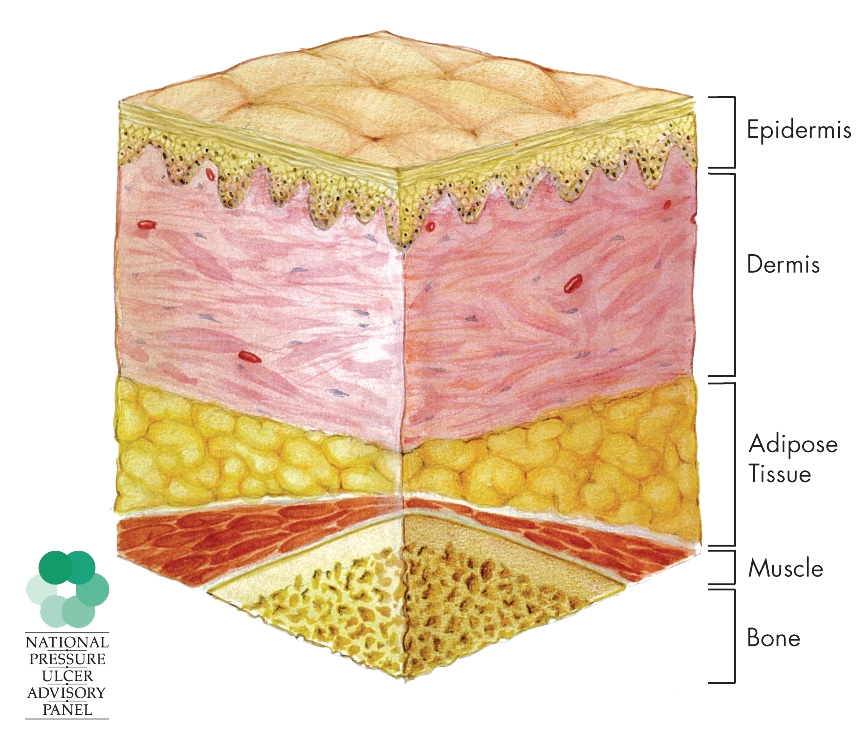
\includegraphics[width=0.33\textwidth]{assets/npuap/normal.png}}

						\subfloat{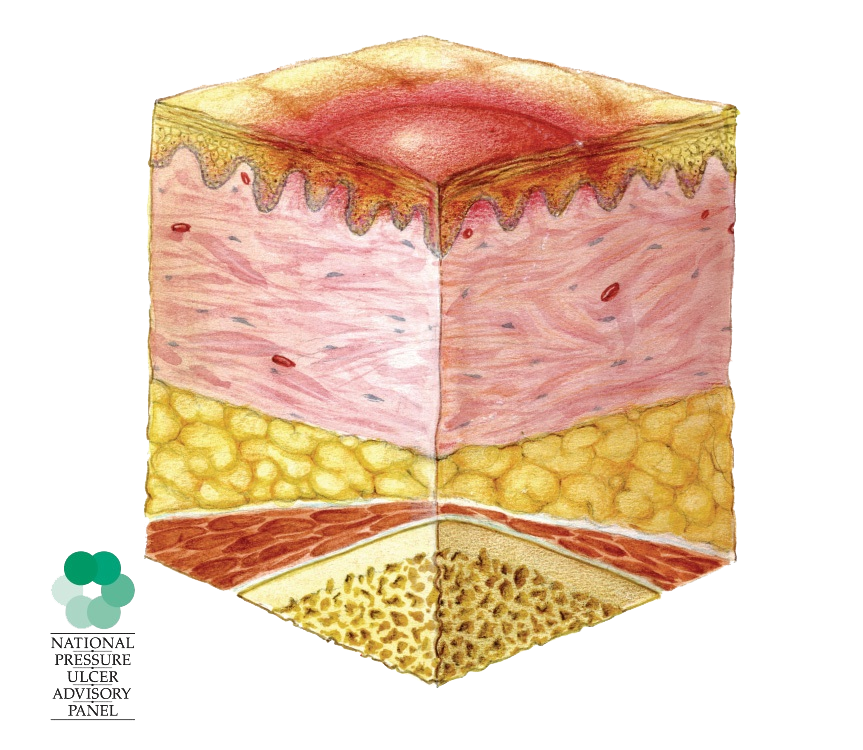
\includegraphics[width=0.33\textwidth]{assets/npuap/stage1.png}}
						\subfloat{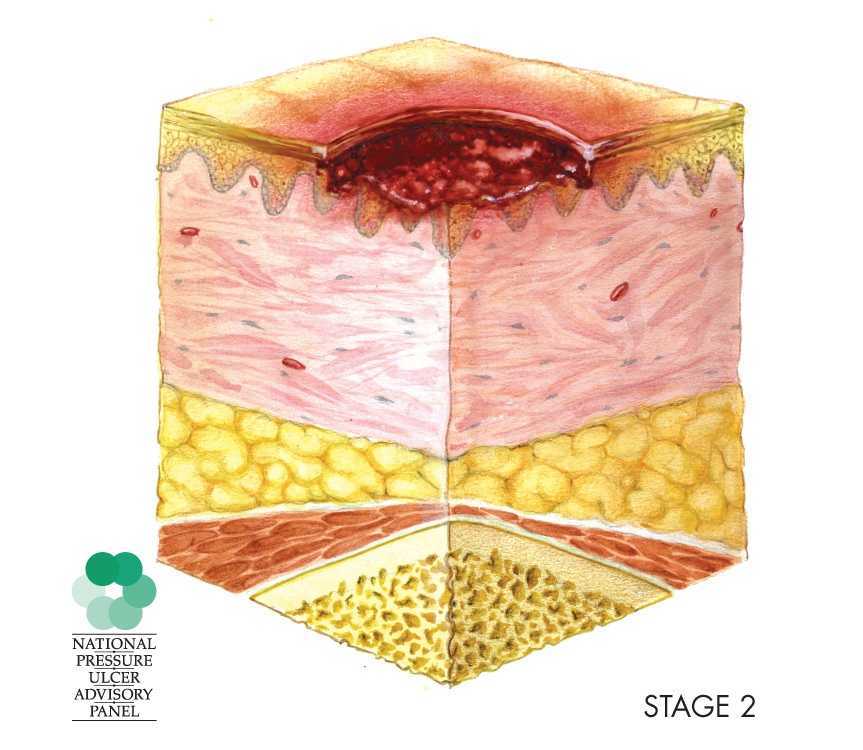
\includegraphics[width=0.33\textwidth]{../latex/assets/npuap/stage2.png}}
						\subfloat{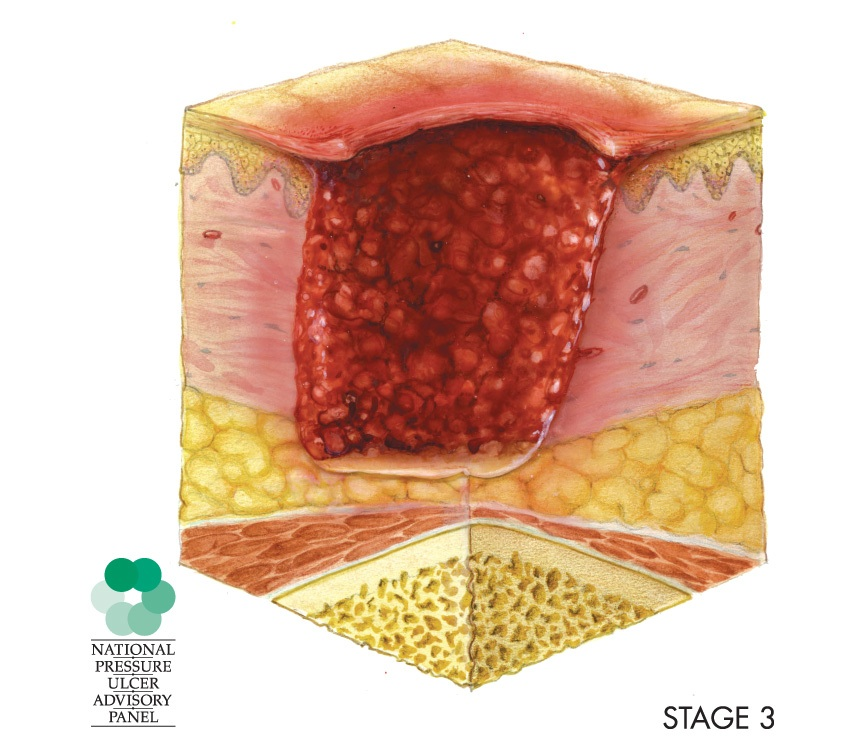
\includegraphics[width=0.33\textwidth]{../latex/assets/npuap/stage3.png}}

						\subfloat{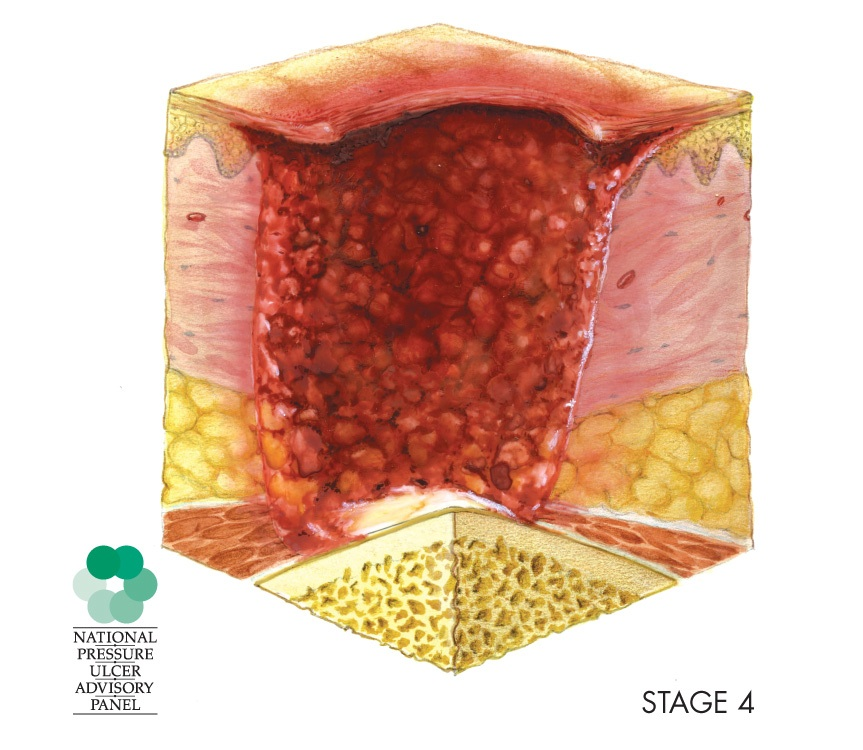
\includegraphics[width=0.33\textwidth]{../latex/assets/npuap/stage4.png}}
						\subfloat{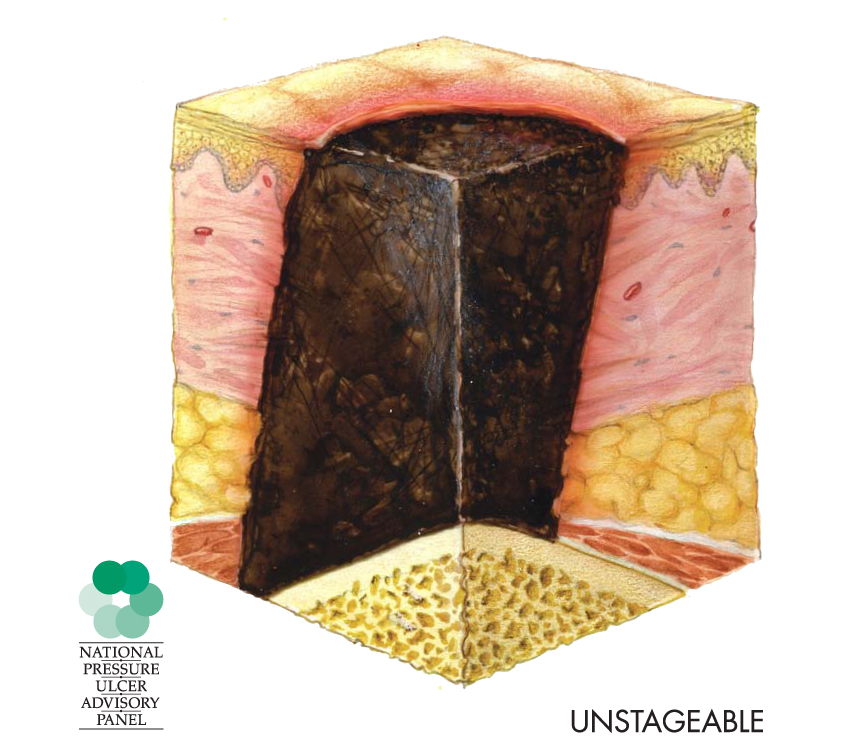
\includegraphics[width=0.33\textwidth]{../latex/assets/npuap/unstageable.png}}
						\subfloat{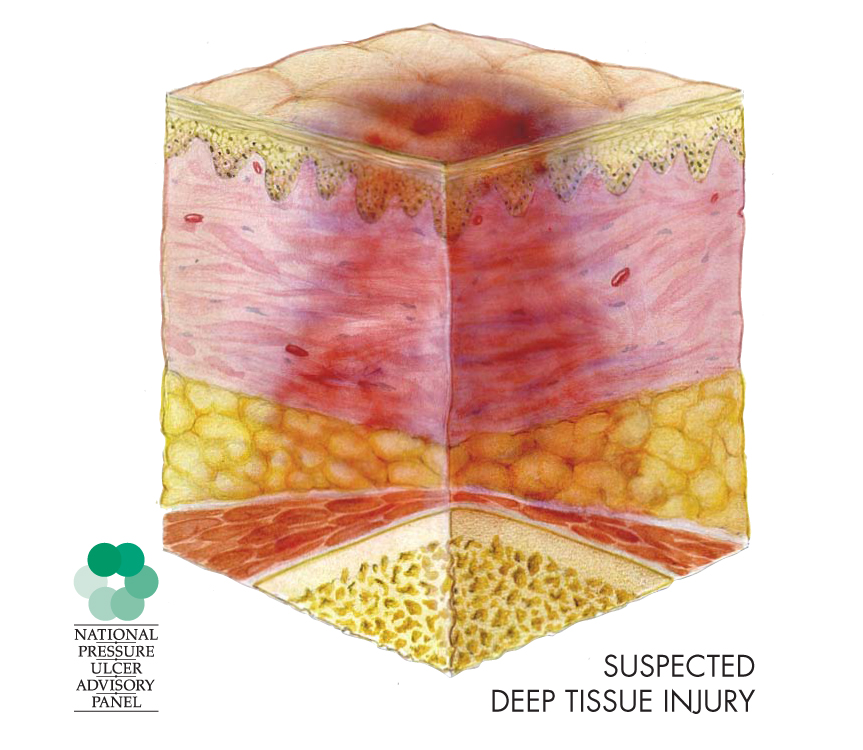
\includegraphics[width=0.33\textwidth]{../latex/assets/npuap/suspectedDTI.png}}

						\caption{\copyright\ National Pressure Ulcer Advisory Panel, used with permission.}
					\end{figure}
			\end{columns}
		\end{frame}